\section{Evaluation}\label{sec:chap04:evaluation}

In this section we evaluate EnDASH and compare its performance with other popular \ac{ABR} algorithms, in terms of \ac{QoE} and energy consumption. We first discuss the methodology that we have adopted.
\subsection{Methodology}
To train and test the throughput engine of EnDASH, we have used a corpus of throughput and power consumption traces collected under user mobility, for both file download and video streaming workloads. These include data collected using Moto G5 and Micromax Canvas Infinity phones over Airtel, Reliance JIO, and Vodafone networks, across five cities in India. The entire corpus is of 39662 seconds of data. The real-life throughput traces are formatted to be compatible with the Mahimahi \cite{mahimahi} network emulation tool. We have divided the collected data set into 70-30 ratio for training and testing. To train the RL algorithms of the buffer length and bitrate decision engine, we have used another  dataset of 57 DASH-ified videos having a total duration of 45 hours. 
The baseline \ac{ABR} streaming algorithms that we have used are \ti{BOLA} \cite{Spiteri2016}, \textit{Pensieve}\cite{mao2017neural}, \textit{Fast MPC} \cite{yin2015control}, and \textit{Robust MPC} \cite{yin2015control}.

\begin{figure}[h]
	\captionsetup[subfigure]{width=0.49\linewidth}
	\begin{center}
		\subfloat[\label{fig:chap04:EnDASH_en}Energy Consumption]{
			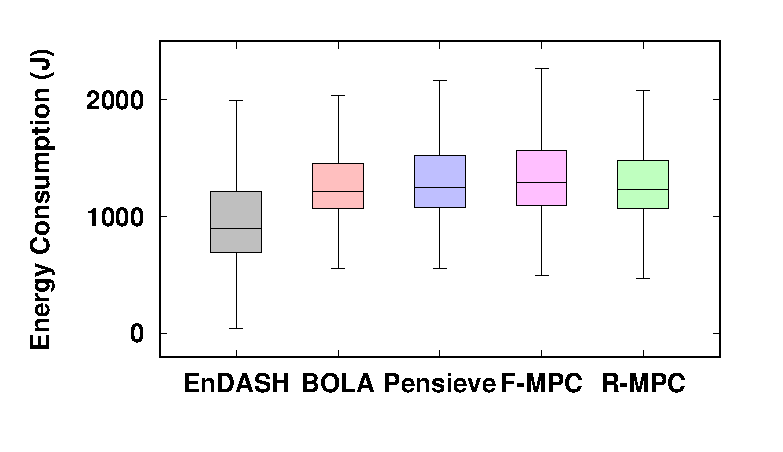
\includegraphics[width=0.33\textwidth]{new_results/simres/Energy}
		}
		\subfloat[\label{fig:chap04:EnDASH_QoE}QoE score (\eqn\ref{eq:chap04:QoE})]{
			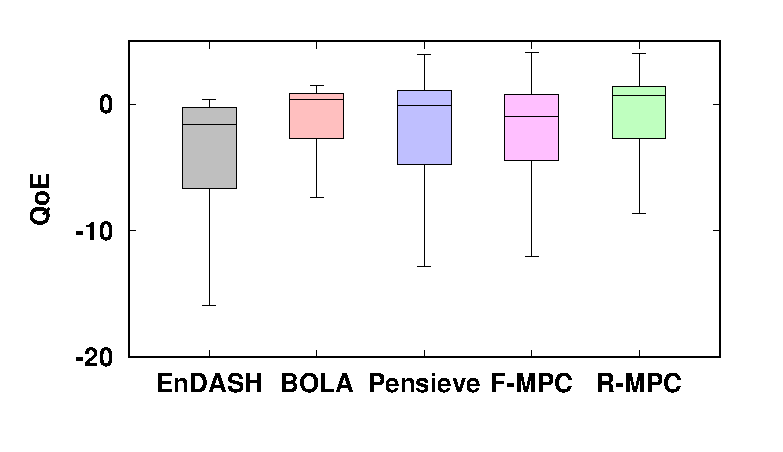
\includegraphics[width=0.33\textwidth]{new_results/simres/QoE}
		}
		\subfloat[\label{fig:chap04:EnDASH_buff}CDF of buffer length]{
			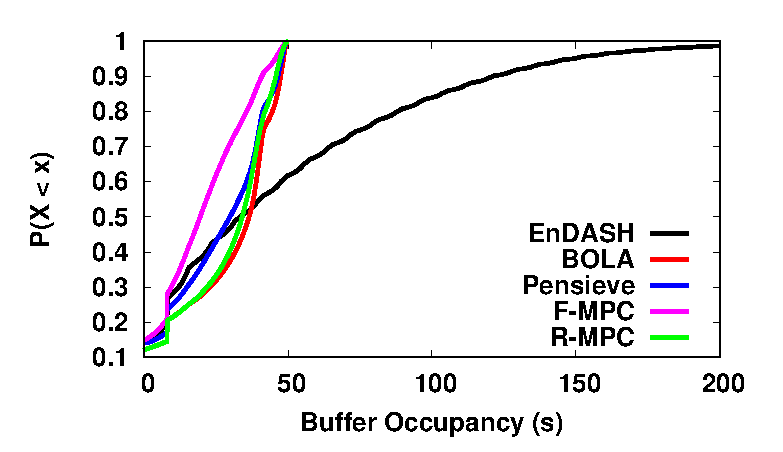
\includegraphics[width=0.33\textwidth]{new_results/simres/BuffOccu}
		}
	\end{center}
	\caption{\label{fig:chap04:EnDASH_vs_others}Performance comparison of EnDASH with baseline \ac{ABR} streaming algorithms, BOLA \cite{Spiteri2016}, Pensieve \cite{mao2017neural}, Fast MPC \cite{yin2015control}, Robust MPC \cite{yin2015control}}
\end{figure}
\begin{figure}[h]
	\captionsetup[subfigure]{width=0.49\linewidth}
	\begin{center}
		\subfloat[\label{fig:chap04:avg_bitrate}Avg. Bitrates in Mbps]{
			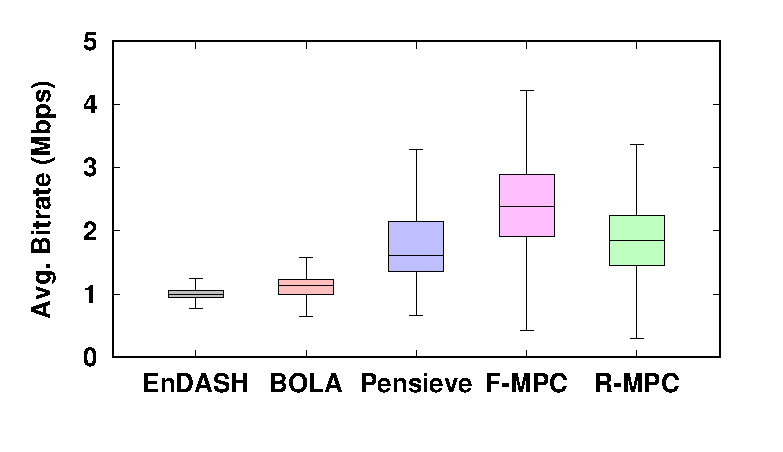
\includegraphics[width=0.49\linewidth]{new_results/simres/AvgBitrate}
		}
		\subfloat[\label{fig:chap04:stall}Stall Time per segment (in seconds))]{
			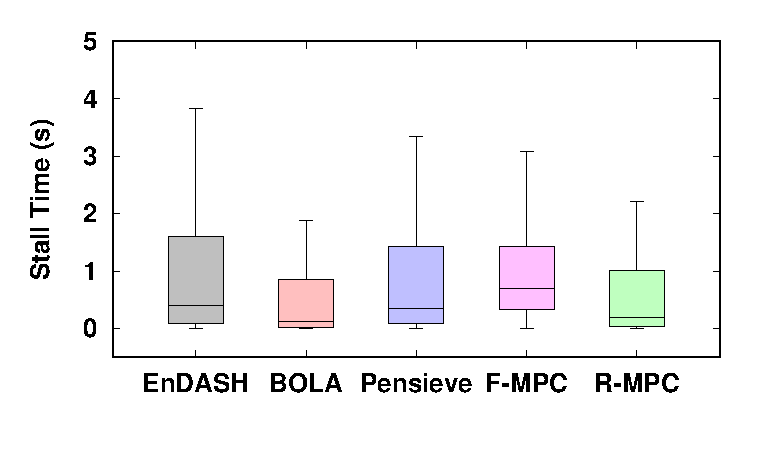
\includegraphics[width=0.49\linewidth]{new_results/simres/Stall}
		}\\
		\subfloat[\label{fig:chap04:smooth}Bitrate Variation]{
			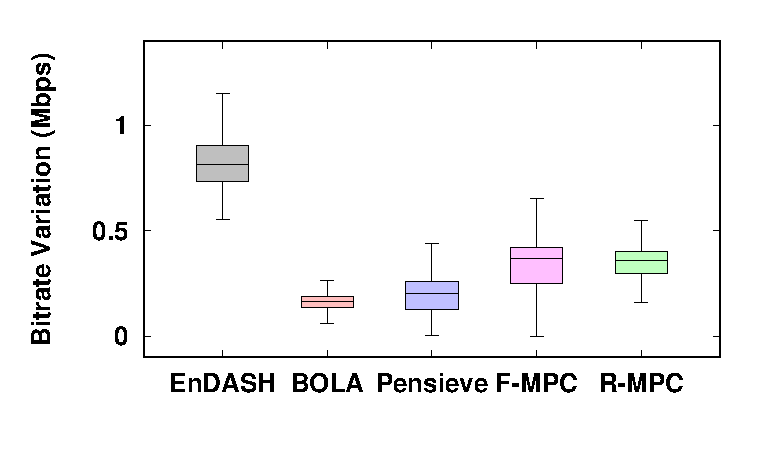
\includegraphics[width=0.49\linewidth]{new_results/simres/BitrateVar}
		}
	\end{center}
	\caption{\label{fig:chap04:indi_QoE}Comparison of different components of \ac{QoE} score (average bitrate, stall time, smoothness) of EnDASH with baseline \ac{ABR} streaming algorithms, BOLA \cite{Spiteri2016}, Pensieve \cite{mao2017neural}, Fast MPC \cite{yin2015control}, Robust MPC \cite{yin2015control}}
\end{figure}

\subsection{EnDASH Versus Baseline ABR Algorithms}
\fig\ref{fig:chap04:EnDASH_vs_others} shows the energy consumption, \ac{QoE} score, and buffer length variation of EnDASH and other baseline \ac{ABR} algorithms. For evaluating these algorithms, the length of each time slot is set to $T=30$ seconds, and the length of the historical window is also set to $x=30$ seconds, i.e., $\prefu{30}{30}$. %So, the average throughput for a prediction window of 30 seconds is predicted using the historical data of 30 seconds. 
In existing literature, the Pensieve \cite{mao2017neural} algorithm has been reported to generate optimal chunk bitrates and video quality. \fig\ref{fig:chap04:EnDASH_en} shows that EnDASH outperforms Pensieve in terms of energy consumption. However, this energy savings comes at the cost of sacrificing the \ac{QoE} with respect to Pensieve as seen in \fig\ref{fig:chap04:EnDASH_QoE}. Moreover, while the average QoE of EnDASH is comparable with the other algorithms, the inter-quartile range of \ac{QoE} is significantly high, implying that the corresponding variability is high.  
 \subsection{QoE Performance Analysis}
To understand the \ac{QoE} performance in detail, we plot the individual components of the \ac{QoE} metric in \fig{\ref{fig:chap04:indi_QoE}}. We observe that the mean of the average bitrate (\fig\ref{fig:chap04:avg_bitrate}) of EnDASH is smaller and its stall time (\fig\ref{fig:chap04:stall}) is comparable with other algorithms. However, the mean bitrate variation (\fig\ref{fig:chap04:smooth}) is much higher. Simultaneously, stall time displays a high variability. The reason for the reduced average bitrate, higher stall time variability, and higher mean of bitrate variation can be attributed to the tuning of the buffer length to the average throughput instead of the instantaneous throughput. For example, if the average throughput predicted is low, the system is forced to download a video chunk at a low bitrate for the entire timeslot, even though the throughput at multiple instances within the timeslot may be high, resulting in lower bitrates. Although the tuning to instantaneous throughput may improve bitrates, it will be associated with higher overhead. Hence, we focus on tuning to average throughput only. Further, the reduced inter-quartile range of the average bitrate is due to the aggressive fetching of video chunks. 
\subsection{Energy Performance Analysis}
EnDASH consumes much less energy because the video chunk download, and hence the playback buffer length, is tuned to the average predicted cellular network throughput. As a result, during high throughput conditions, the playback buffer length will increase, thereby facilitating the download of a higher number of chunks in a slot. This consecutive fetching of chunks reduces the tail energy which eventually manifests in the reduction of overall energy consumption as seen in \fig\ref{fig:chap04:EnDASH_en}. The resulting trade-off is reflected in the increase in buffer length in comparison with the buffer length of competing ABR algorithms.  \fig\ref{fig:chap04:EnDASH_buff} shows the CDF of playback buffer length of different algorithms. It is seen that while the maximum buffer length of existing algorithms is 50 seconds that of EnDASH can go up to 200 seconds; but this is a rare instance. In nearly 60\% of the time the buffer length remains below 50 seconds.

\begin{figure}[ht]%
	\centering
	{\fbox{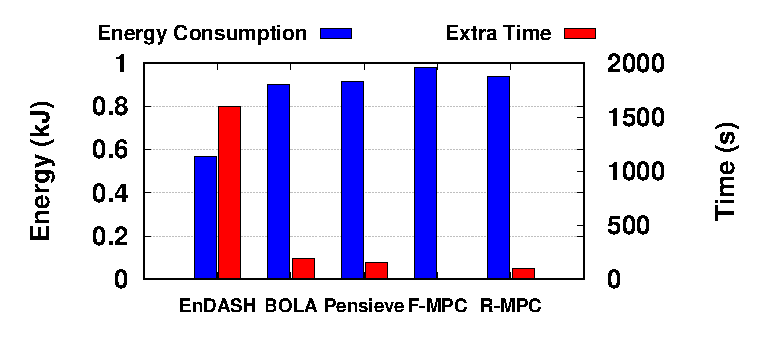
\includegraphics[width=0.7\linewidth]{new_results/simres/EnergyConsumption}}}	
	\caption{Energy Consumption and Extra Playtime obtained w.r.t. Fast MPC, which has the highest energy consumption}\vspace*{-0.5cm}
	\label{fig:chap04:vid_time_save}
\end{figure}
\subsection{Gain from Energy Savings}
\indent In this section, we discuss the gain in video playback time achieved by using EnDASH. FastMPC has the highest energy consumption among all algorithms. \fig{\ref{fig:chap04:vid_time_save}} shows the gain in video playback time achieved by the algorithms with respect to FastMPC while streaming a 2200 second video. It shows that using the energy saved by streaming the video using EnDASH, one can gain an additional 1403 seconds and 1440 seconds of video playback time in comparison with BOLA and Pensieve, respectively. Thus, one may infer that EnDASH can be used as a potential ABR streaming algorithm for increasing battery backup in smartphones.

\subsection{Feature Importance Study on Throughput Prediction Engine} The primary objective of the throughput prediction engine is to account for the impact of cellular network technology change, i.e., the switching between 2G, 3G, 4G, etc., on network throughput.
\fig{\ref{fig:chap04:feature_imp}} shows the feature importance of different input parameters when predicting throughput. We observe that vertical handovers and associated technology (Network Type) have the highest weightage among all parameters, 0.32 and 0.21, respectively. The importance of such features in throughput prediction points out to
the absolute necessity of considering the existence of legacy systems when designing algorithms for 4G networks. 
\begin{figure}[!ht]
    \centering
    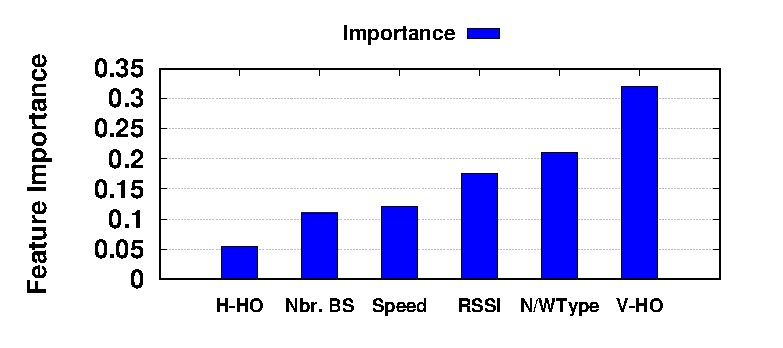
\includegraphics[width=0.7\linewidth]{new_results/simres/FeatureImpotance}
    \caption{Feature importance of the input parameters; signal strength, associated technology, and handovers (HOs)) between technology are the three features having the highest contribution in deciding throughput}\vspace*{-0.5cm}
    \label{fig:chap04:feature_imp}
\end{figure}
\begin{figure}[ht]
	\captionsetup[subfigure]{width=0.49\linewidth}
	\begin{center}
		\subfloat[\label{fig:chap04:MAPE_diff_scene}MAPE score measuring error of throughput prediction in different regions for various combinations of considering  associated technology and vertical handover (HO); for $\prefu{30}{30}$]{
			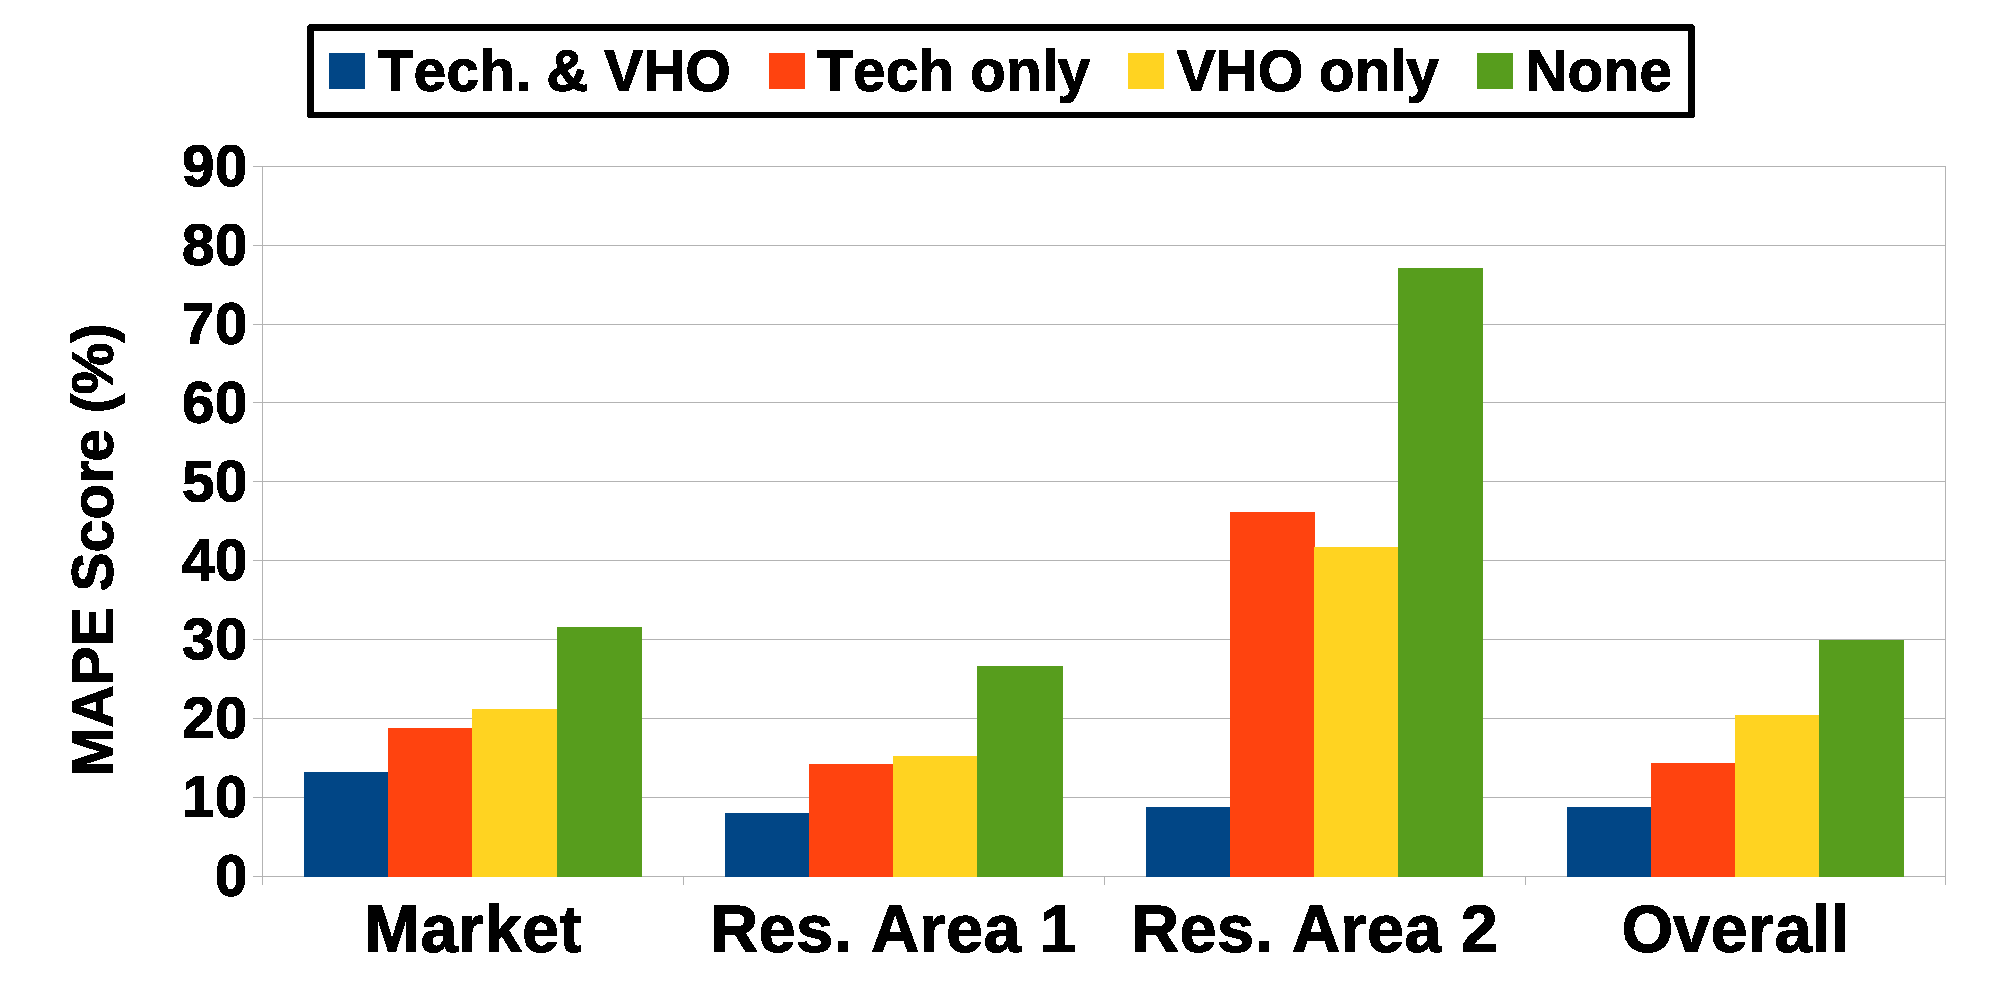
\includegraphics[width=0.49\linewidth]{figures/resi_vs_market_vs_overall_MAPE.eps}
		}
		\subfloat[\label{fig:chap04:Perf_VHO}Impact of considering associated technology and vertical handovers (HOs) on performance metrics of EnDASH; for $\prefu{30}{30}$]{
			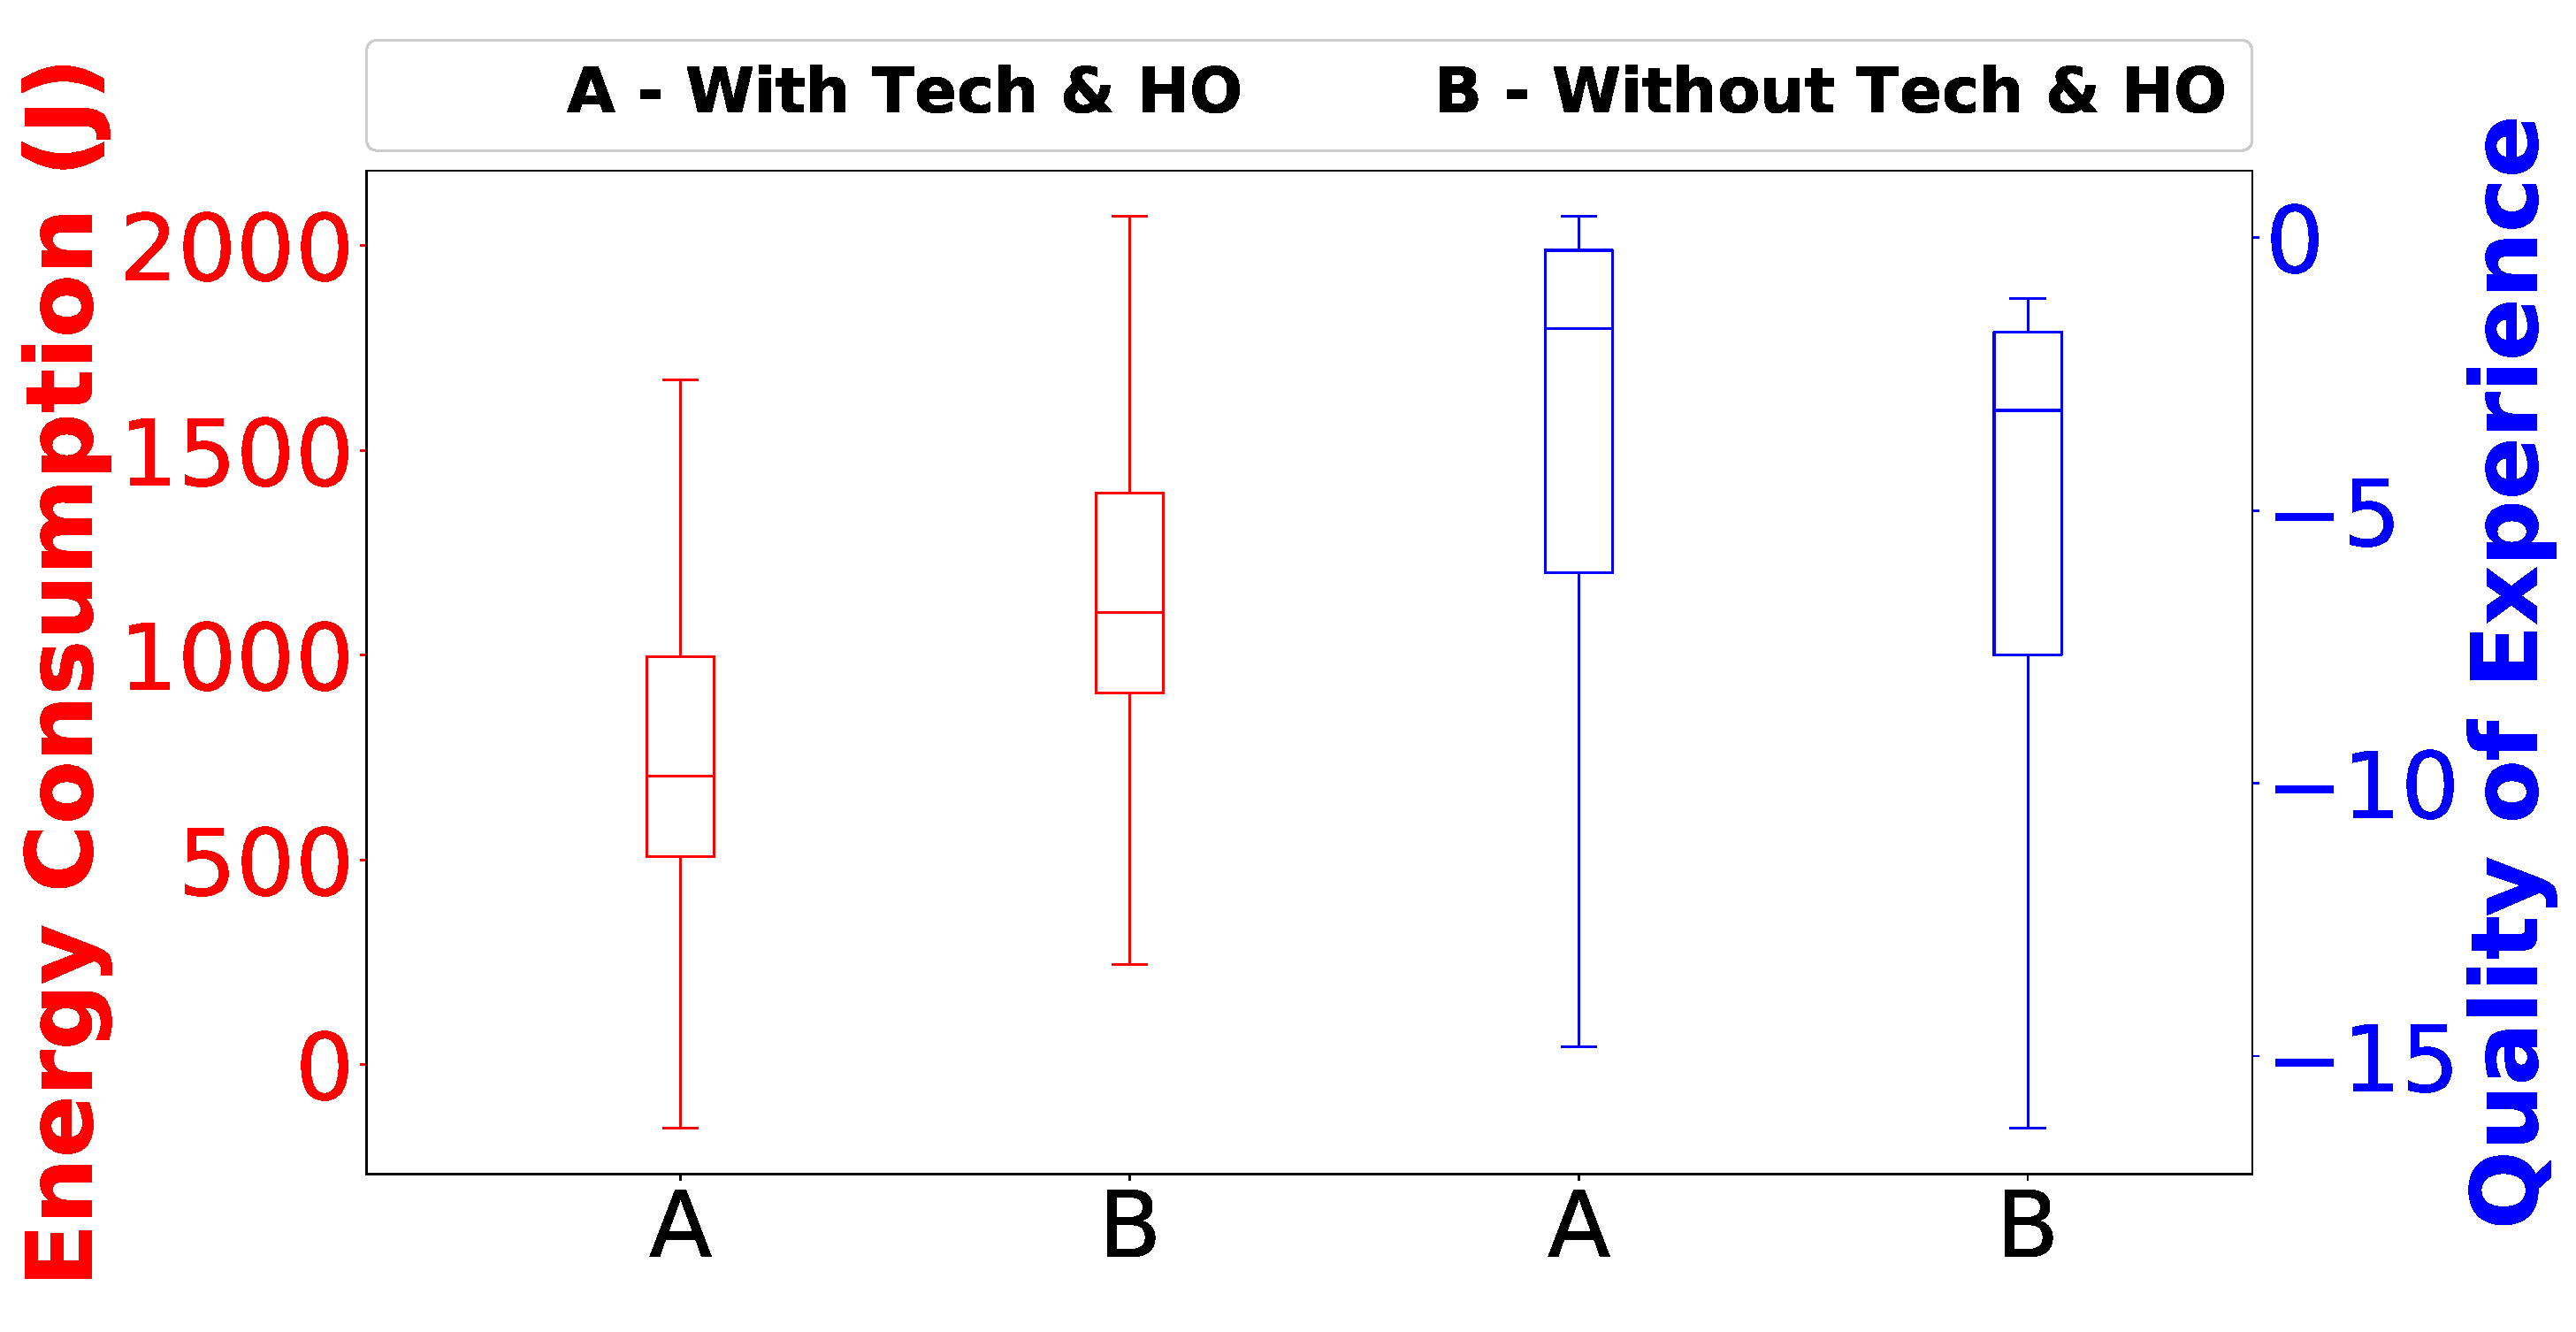
\includegraphics[width=0.49\linewidth]{figures/pow_qoe_comp.eps}
		}\\
		\subfloat[\label{fig:chap04:thpt_pred_trace}Predicted vs Actual throughput using the RF algorithm when associated technology and vertical handover (HO) is considered]{
			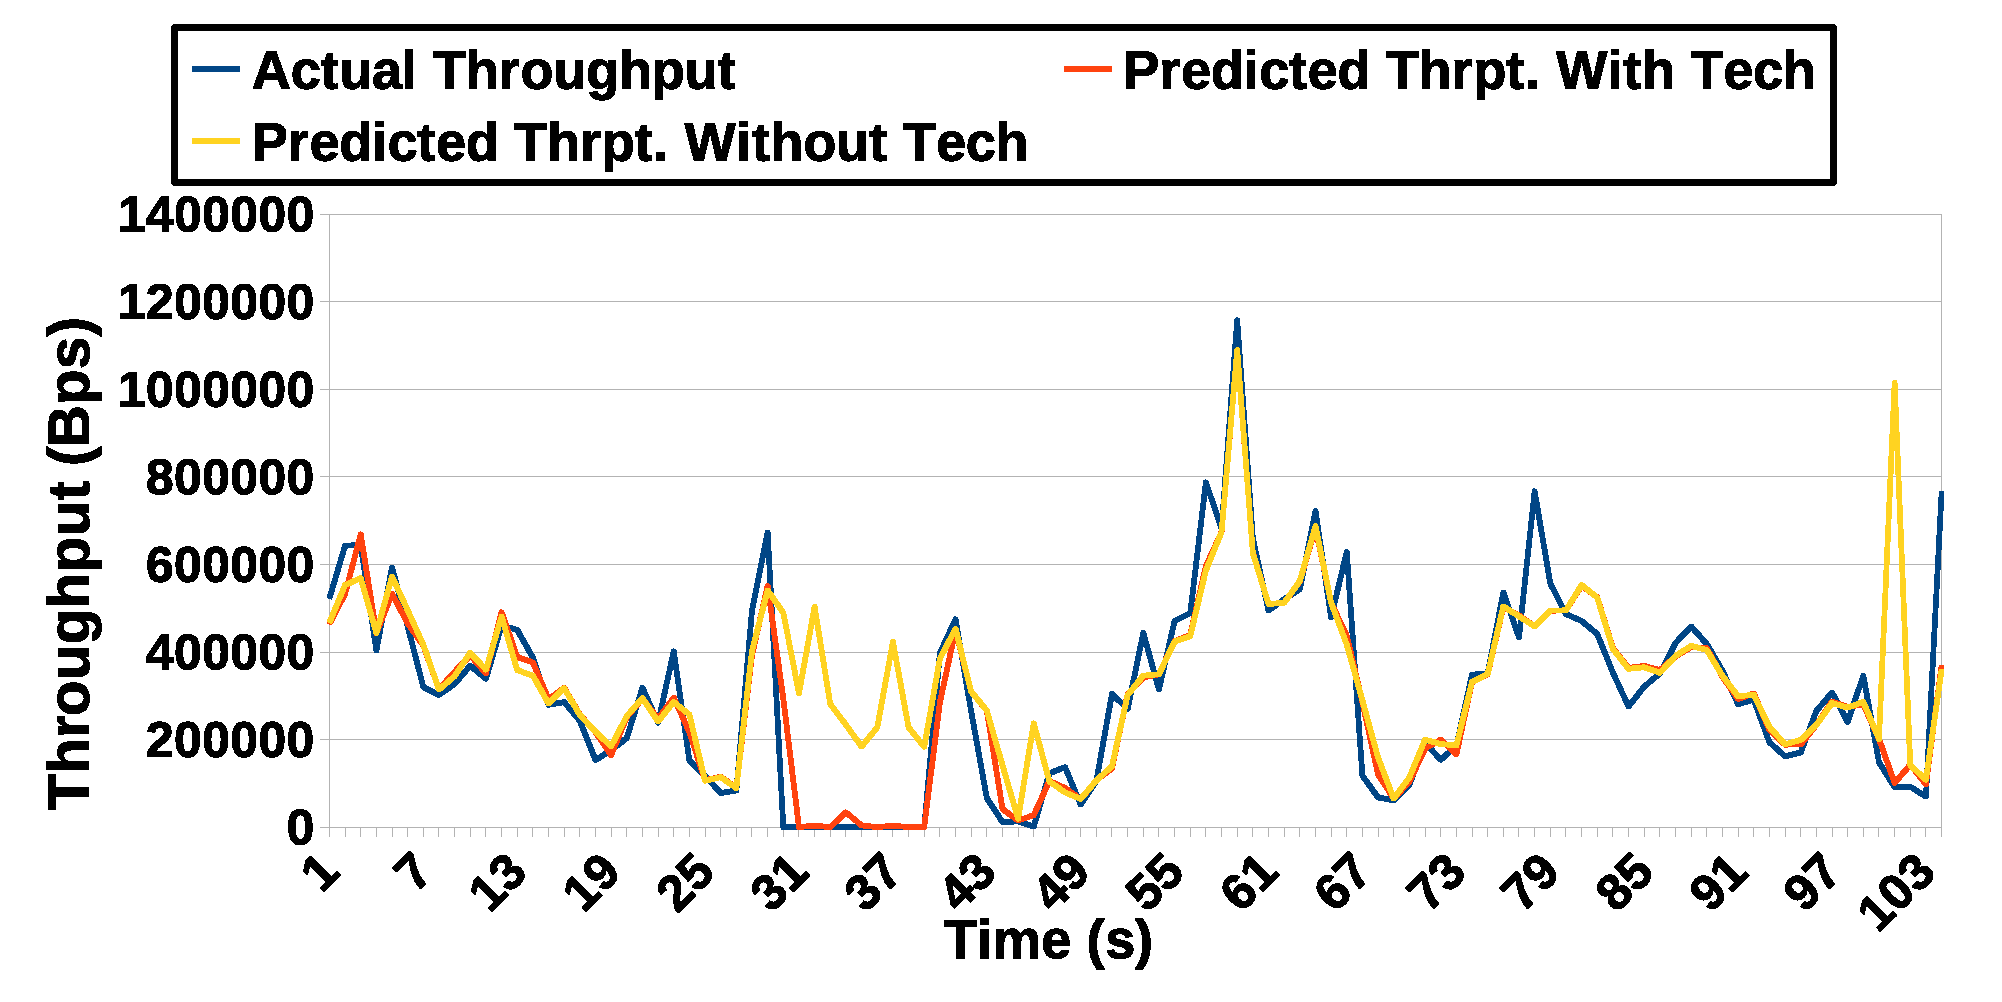
\includegraphics[width=0.49\linewidth]{figures/predicted_vs_actual_vs_Tech.eps}
		}
	\end{center}
	\caption{Effect of Associated Technology and Vertical Handovers (HOs) on Throughput Prediction and EnDASH performance for $\prefu{30}{30}$}
\end{figure}
%  \begin{figure*}[t]%
%\centering
%\subfigure[MAPE score measuring error of throughput prediction in different regions for various combinations of considering  associated technology and vertical handover (HO); for $\prefu{30}{30}$]{%
%\label{fig:MAPE_diff_scene}%
%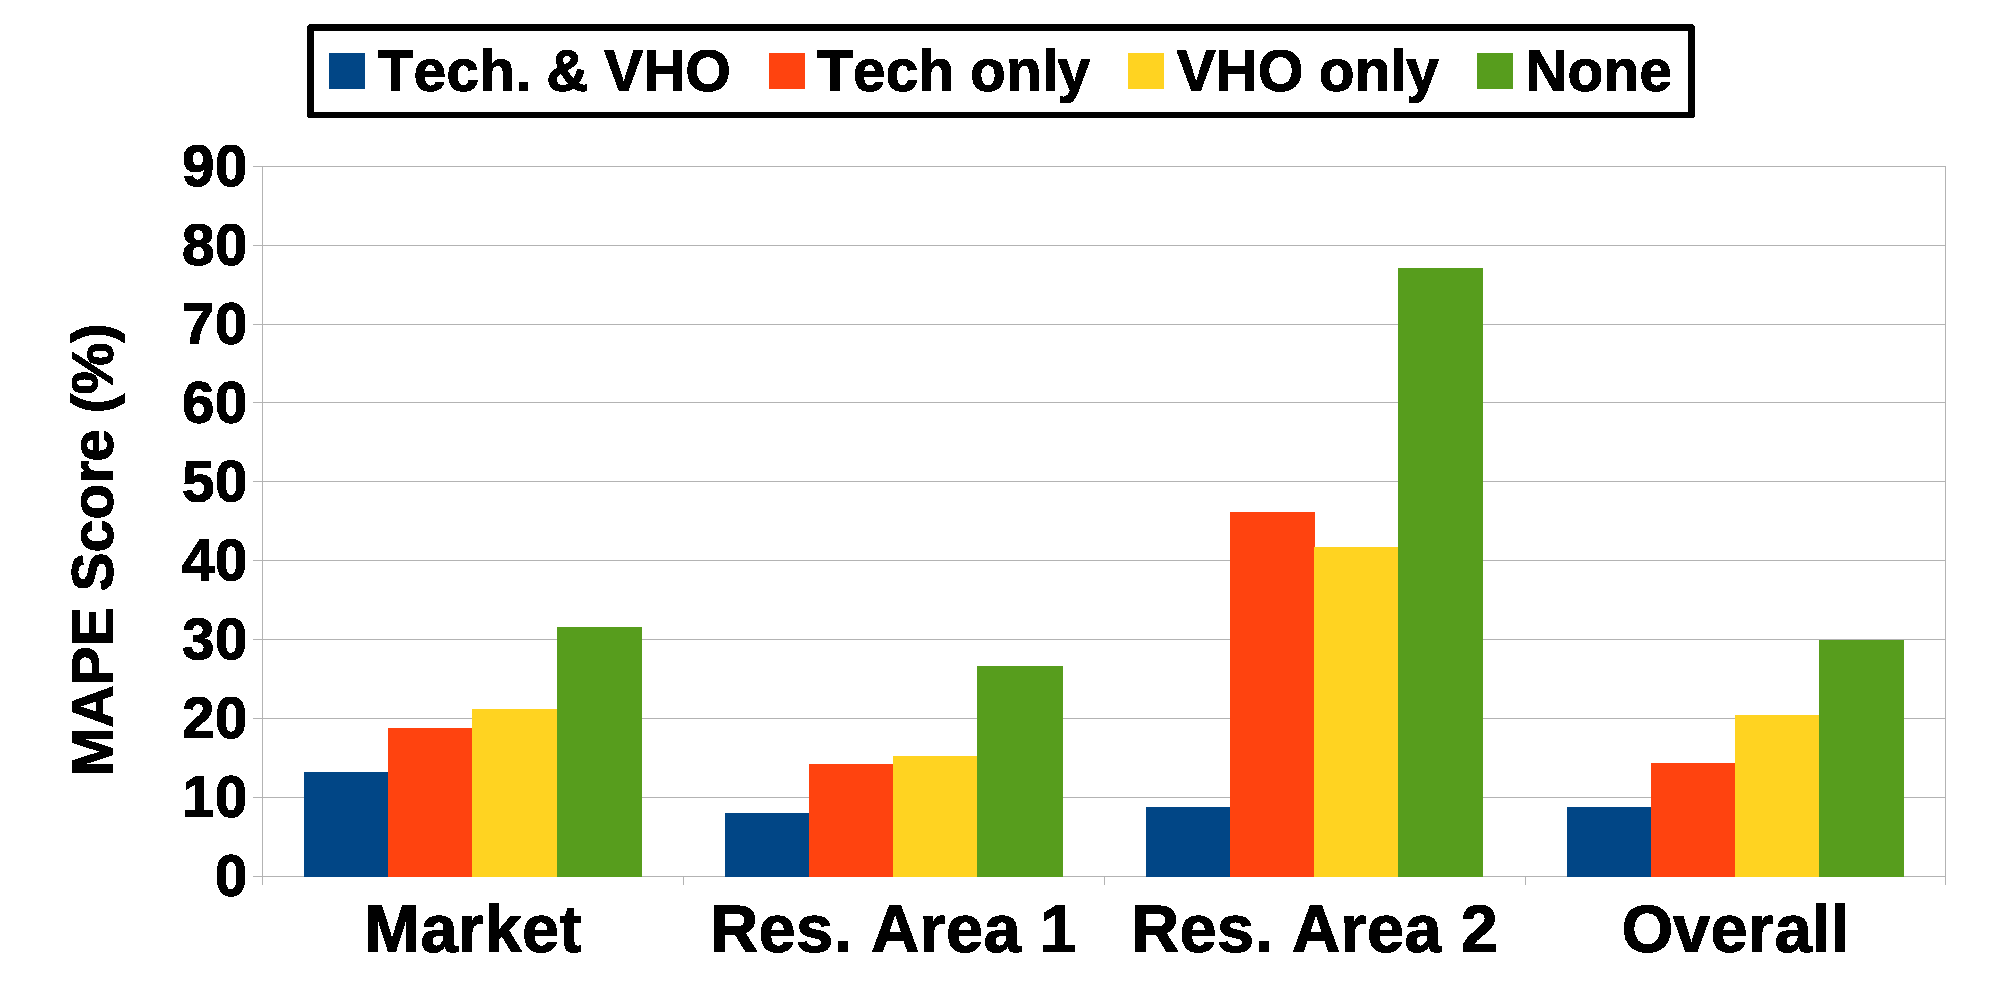
\includegraphics[width=0.3\textwidth]{figures/resi_vs_market_vs_overall_MAPE.eps}}
%\hspace{0.1cm}
%\subfigure[Impact of considering associated technology and vertical handovers (HOs) on performance metrics of EnDASH; for $\prefu{30}{30}$]{%
%\label{fig:Perf_VHO}%
%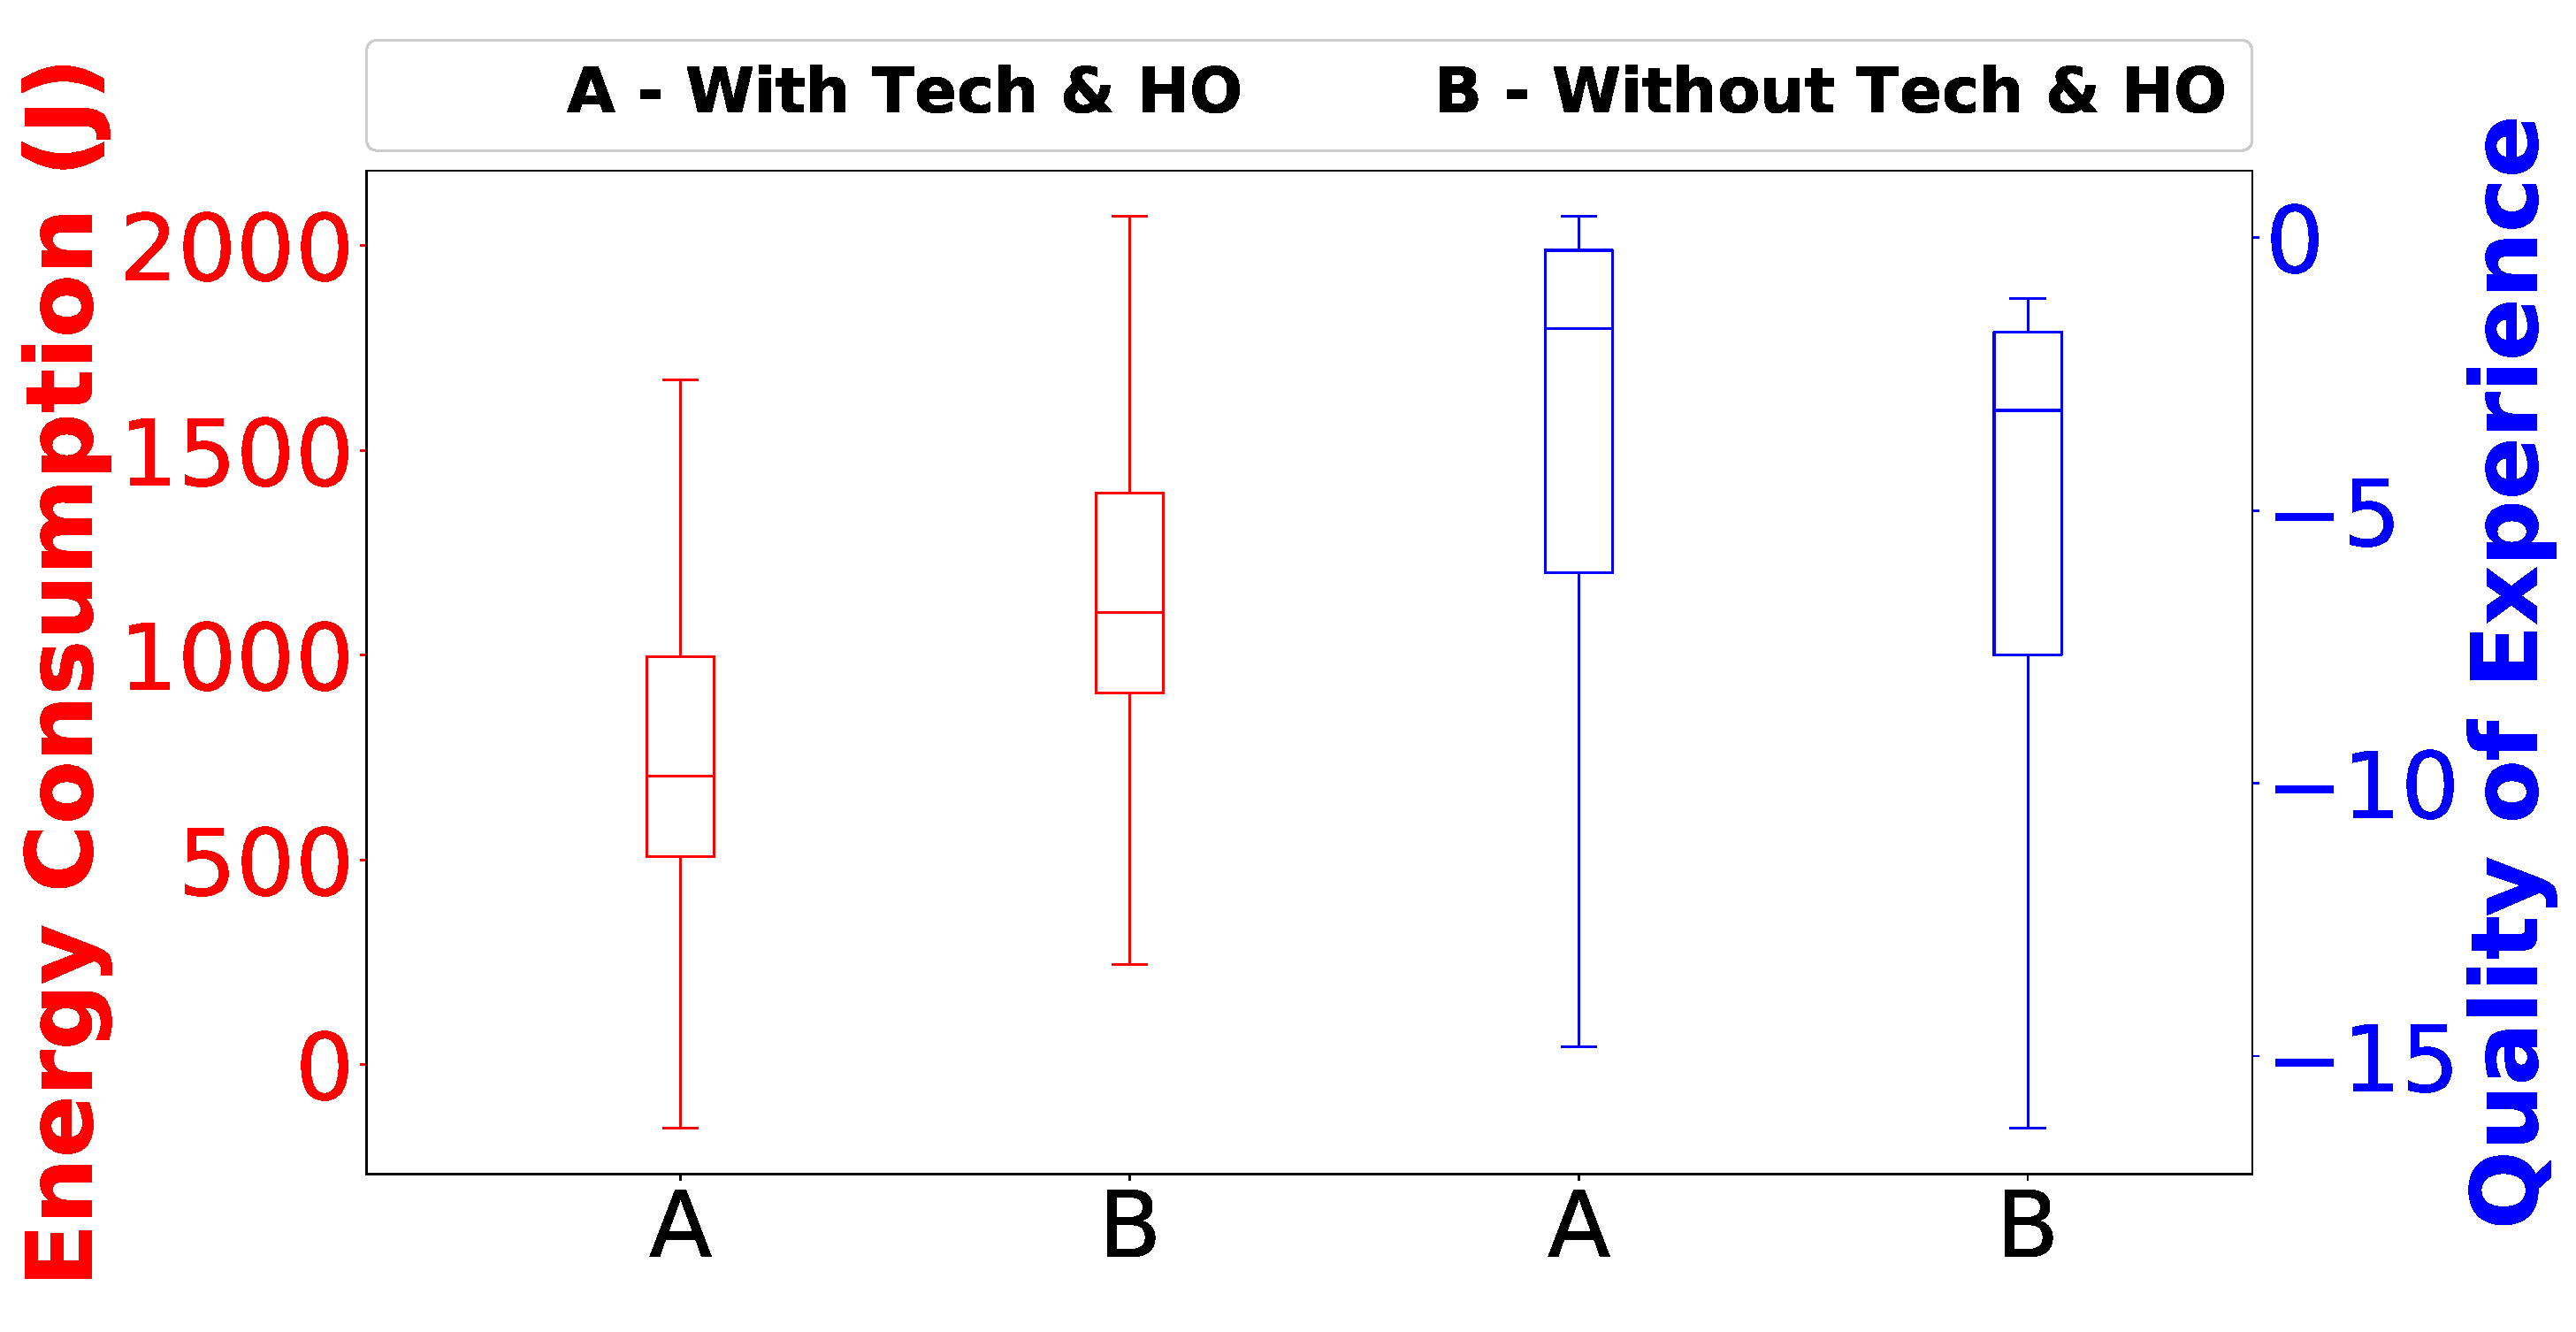
\includegraphics[width=0.3\textwidth]{figures/pow_qoe_comp.eps}}%
%\hspace{0.1cm}
%\subfigure[Predicted vs Actual throughput using the RF algorithm when associated technology and vertical handover (HO) is considered.]{%
%\label{fig:thpt_pred_trace}%
%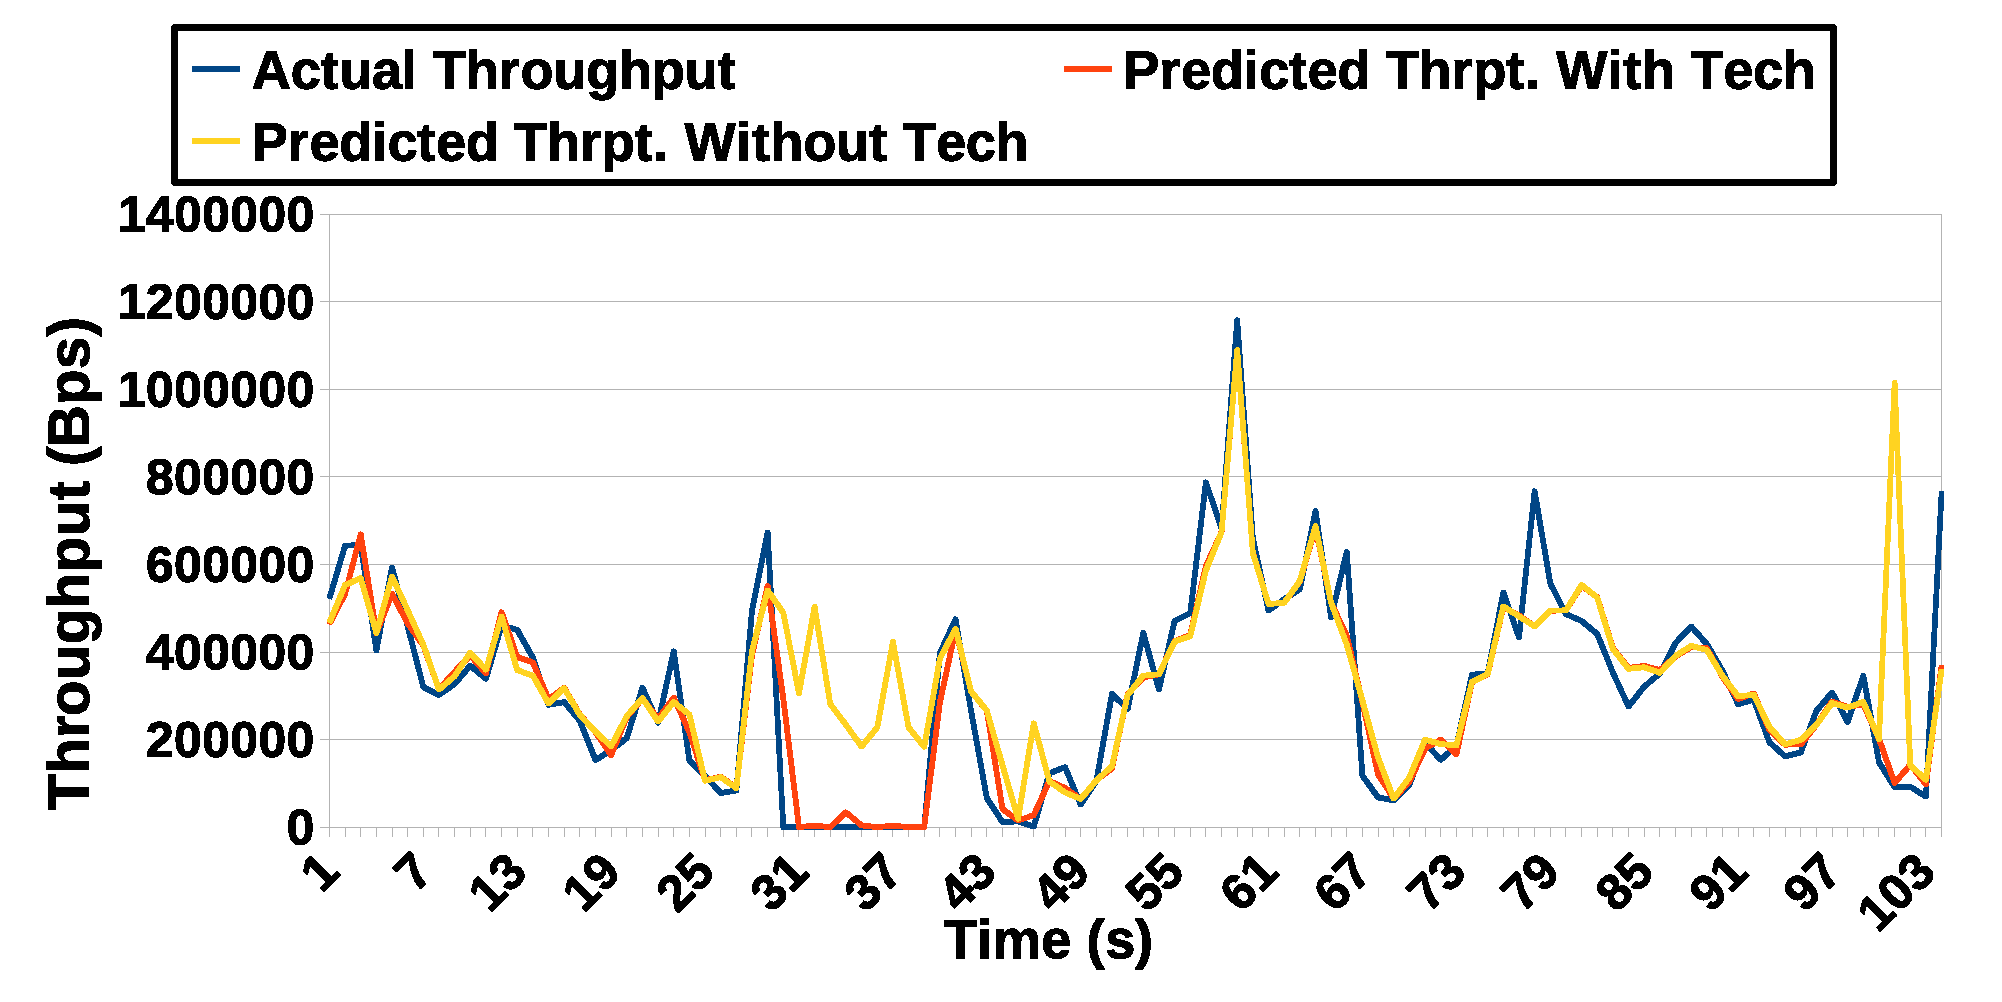
\includegraphics[width=0.3\textwidth]{figures/predicted_vs_actual_vs_Tech.eps}}%
%\caption{Effect of Associated Technology and Vertical Handovers (HOs) on Throughput Prediction and EnDASH performance for $\prefu{30}{30}$}\vspace*{-0.5cm}
%\end{figure*}
\subsection{Importance of Associated Technology}
\indent To understand the impact of associated technology and vertical handovers on the throughput prediction error, we have evaluated the MAPE~\footnote{\indent MAPE score, which quantifies error in throughput prediction,  is:
\begin{align}
\text{MAPE\ score} = \frac{1}{N}\sum_{i=1}^N\left|\frac{\tau_i-\hat{\tau}_i}{\tau_i}\right|\times 100\%
\end{align}
where $\tau_i$ and $\hat{\tau}_i$ respectively denote actual and  predicted throughput in the $\mathrm{i^{th}}$ timeslot.
} score over different regions. For this, we have divided the data traces collected in Kharagpur into three categories - (a) crowded Market Place, (b) a residential area with extensive 4G coverage (Residential Area 1), and (c) a residential area with limited 4G coverage (Residential Area 2). The overall MAPE score and the MAPE score for the three different scenarios, each with different combinations of associated network technology and vertical handover, is shown in \fig{\ref{fig:chap04:MAPE_diff_scene}}. It is observed that the lowest MAPE score is reported when the throughput prediction considers the associated technologies and vertical handovers, especially when 4G coverage is limited. 
\fig{\ref{fig:chap04:Perf_VHO}} shows how the inclusion of both associated technology and vertical handover as features in the throughput prediction improves the EnDASH performance, in terms of energy consumption as well as \ac{QoE}.\\
\indent The impact of associated technology can be further understood if we look into the actual throughput traces and its prediction, which \fig{\ref{fig:chap04:thpt_pred_trace}} shows.
We have generated  \fig{\ref{fig:chap04:thpt_pred_trace}} with $\prefu{30}{30}$.
It is observed that if the associated technology and the vertical handover is not considered then there is significant mismatch in low throughput regions where there is a tendency of over estimation of the throughput.
